\chapter{Energy, Momentum, and the Electromagnetic Field}

The final lecture begins with a repair and ends with the object that will
stand on the right-hand side of Einstein's equation. The route is not a
detour. A sign convention for the electric field must first be made
explicit; three distinct meanings of momentum must then be separated.
Only after those preliminaries can field theory be read as ordinary
mechanics with one degree of freedom at every point in space. The
Hamiltonian, local energy density, Noether momentum, electromagnetic
energy, and Poynting vector then follow in one continuous argument.

\section{A Convention That Must Be Carried Consistently}

The preliminary notes were to be posted for the class, but the issue is
important enough to settle aloud. Byron had noticed an inconsistency not
within the course notation, but between that notation and the notation
used almost everywhere else. This is an occupational hazard of deriving
equations afresh: an internally consistent private convention can drift
away from the public one.

Write \(\mathbf E_M\) for the standard Maxwell--Franklin convention and
\(\mathbf E_L\) for the convention used in the preceding lectures. With
the course's covariant component \(A_0\), they are
\begin{align}
\mathbf E_M
  &= -\dot{\mathbf A}+\boldsymbol{\nabla}A_0,
&
\mathbf E_L
  &= +\dot{\mathbf A}-\boldsymbol{\nabla}A_0
   =-\mathbf E_M .
\label{eq:two-electric-conventions}
\end{align}
Many books instead introduce the scalar potential
\(\Phi=-A_0\); then the first formula reads
\(\mathbf E_M=-\dot{\mathbf A}-\boldsymbol{\nabla}\Phi\).
The magnetic field does not change:
\begin{equation}
\mathbf B=\boldsymbol{\nabla}\times\mathbf A.
\label{eq:B-from-A-opening}
\end{equation}

In rationalized units with \(c=1\), the standard Maxwell--Franklin
equations are
\begin{align}
\boldsymbol{\nabla}\times\mathbf E_M&=-\dot{\mathbf B},
&
\boldsymbol{\nabla}\cdot\mathbf B&=0,
\nonumber\\
\boldsymbol{\nabla}\times\mathbf B&=\dot{\mathbf E}_M+\mathbf J_F,
&
\boldsymbol{\nabla}\cdot\mathbf E_M&=\rho_F .
\label{eq:maxwell-franklin}
\end{align}
Benjamin Franklin's historical choice fixes the sign of charge: the
electron is negative in this convention. The course convention also
reverses the source labels,
\begin{equation}
\mathbf J_L=-\mathbf J_F,
\qquad
\rho_L=-\rho_F.
\label{eq:source-convention-map}
\end{equation}
Substitution of
\(\mathbf E_L=-\mathbf E_M\) therefore gives
\begin{align}
\boldsymbol{\nabla}\times\mathbf E_L&=+\dot{\mathbf B},
&
\boldsymbol{\nabla}\cdot\mathbf B&=0,
\nonumber\\
\boldsymbol{\nabla}\times\mathbf B&=-\dot{\mathbf E}_L-\mathbf J_L,
&
\boldsymbol{\nabla}\cdot\mathbf E_L&=\rho_L .
\label{eq:maxwell-course-convention}
\end{align}

\begin{figure}[H]
\centering

\includegraphics[width=\linewidth]{../../figures/lecture_10_figure_01.png}
\caption{The complete board comparison between the Maxwell--Franklin and
course conventions.}
\par\smallskip
\textit{Lecture frame: 00:07:10.}
\end{figure}

Nothing measurable depends on which dictionary is chosen. What matters
is consistency, especially when a calculated field is compared with a
published experimental value. The practical joke is that such direct
numerical comparisons had arisen so rarely in the lecturer's own work
that the opposite sign survived unnoticed until the class called
attention to it. For the electromagnetic calculation later in this
chapter we shall use the standard field
\(\mathbf E\equiv\mathbf E_M\).

\section{Three Different Quantities Called Momentum}

The word \emph{momentum} now has to be unpacked. Mechanical momentum,
canonical momentum, and Noether momentum can coincide in simple
problems, but they are not three descriptions of one quantity. In a
general system they can have different numerical values.

\subsection{Mechanical momentum}

For a body of total mass \(M\), mechanical momentum is
\begin{equation}
\mathbf P_{\mathrm{mech}}=M\dot{\mathbf X}_{\mathrm{cm}}.
\label{eq:mechanical-momentum}
\end{equation}
For one particle, \(\mathbf X_{\mathrm{cm}}\) is simply its position.
For a composite body, the center-of-mass qualification is essential.

\begin{figure}[H]
\centering

\includegraphics[width=\linewidth]{../../figures/lecture_10_figure_02.png}
\caption{Mechanical momentum introduced as mass times the
center-of-mass velocity.}
\par\smallskip
\textit{Lecture frame: 00:11:15.}
\end{figure}

\subsection{Canonical momentum}

Suppose the mechanics is described by
\(L(q_i,\dot q_i)\). The canonical momentum conjugate to \(q_i\) is
\begin{equation}
p_i=\frac{\partial L}{\partial\dot q_i}.
\label{eq:canonical-momentum}
\end{equation}
For
\begin{equation}
L=\frac12 m\dot{\mathbf x}^{\,2}-V(\mathbf x),
\label{eq:simple-particle-lagrangian}
\end{equation}
this gives \(\mathbf p=m\dot{\mathbf x}\), so canonical and mechanical
momentum happen to agree.

\begin{figure}[H]
\centering

\includegraphics[width=\linewidth]{../../figures/lecture_10_figure_03.png}
\caption{Mechanical and canonical momentum displayed beside the simple
particle Lagrangian.}
\par\smallskip
\textit{Lecture frame: 00:13:40.}
\end{figure}

A charged particle in a magnetic field is the useful counterexample.
With the sign convention written on the board,
\begin{equation}
L=\frac12m\dot{\mathbf x}^{\,2}-V(\mathbf x)
  -e\,\dot{\mathbf x}\cdot\mathbf A(\mathbf x),
\label{eq:magnetic-particle-lagrangian}
\end{equation}
and therefore
\begin{equation}
p_i=m\dot x_i-eA_i.
\label{eq:magnetic-canonical-shift}
\end{equation}
Changing the convention for charge or for the interaction term changes
the displayed sign, but not the lesson: the canonical momentum contains
a vector-potential contribution and is not merely \(m\dot x_i\).
Hamilton's equations use the canonical variable. One may later move the
field-dependent term to the other side of an equation and recover a
Newtonian-looking acceleration, but that rearrangement does not change
the definition.

\begin{figure}[H]
\centering

\includegraphics[width=\linewidth]{../../figures/lecture_10_figure_04.png}
\caption{The vector-potential term shifts canonical momentum away from
mechanical momentum.}
\par\smallskip
\textit{Lecture frame: 00:15:50.}
\end{figure}

\subsection{Noether momentum}

The third momentum is the conserved charge associated with spatial
translation invariance. For an infinitesimal symmetry
\begin{equation}
q_i\longrightarrow q_i+\delta q_i
\end{equation}
that leaves the Lagrangian invariant, Noether's theorem gives, up to the
normalization of the infinitesimal parameter,
\begin{equation}
Q=\sum_i p_i\,\delta q_i.
\label{eq:noether-charge-mechanics}
\end{equation}
The \(p_i\) appearing here are canonical momenta. If the symmetry is a
uniform translation and canonical momentum happens to equal mechanical
momentum, \(Q\) reduces to the familiar total momentum. In a less simple
system that coincidence must be proved, not assumed.

\begin{figure}[H]
\centering

\includegraphics[width=\linewidth]{../../figures/lecture_10_figure_05.png}
\caption{The Noether charge assembled from canonical momenta and the
infinitesimal changes of the coordinates.}
\par\smallskip
\textit{Lecture frame: 00:19:00.}
\end{figure}

\section{Energy as the Hamiltonian}

Spatial translations lead to momentum; time translations lead to
energy. If the Lagrangian has no explicit time dependence, the
Hamiltonian
\begin{equation}
H=\sum_i p_i\dot q_i-L
\label{eq:hamiltonian-definition}
\end{equation}
is conserved. This is the Legendre transform of the Lagrangian, not a
rule about changing signs by inspection.

\begin{figure}[H]
\centering

\includegraphics[width=\linewidth]{../../figures/lecture_10_figure_06.png}
\caption{The Hamiltonian written as the Legendre transform of a general
Lagrangian.}
\par\smallskip
\textit{Lecture frame: 00:22:55.}
\end{figure}

For the one-particle example,
\begin{align}
p&=m\dot x,
\nonumber\\
H&=p\dot x-L
  =m\dot x^2-\left(\frac12m\dot x^2-V(x)\right)
  =\frac12m\dot x^2+V(x).
\label{eq:particle-hamiltonian}
\end{align}
Thus the Lagrangian is kinetic minus potential energy, whereas the
Hamiltonian is kinetic plus potential energy.

\begin{figure}[H]
\centering

\includegraphics[width=\linewidth]{../../figures/lecture_10_figure_07.png}
\caption{The particle calculation showing how
\(H=T+V\) follows from \(H=p\dot x-L\).}
\par\smallskip
\textit{Lecture frame: 00:24:20.}
\end{figure}

When every velocity dependence is a conventional positive quadratic
kinetic term and the remainder contains no velocities, one can read off
the Hamiltonian by reversing the sign of the nonvelocity part. That
shortcut will be used repeatedly. It is safe only because the Legendre
transform has this simple form in the examples at hand.

\section{A Field Is a Mechanical System with Continuously Many Coordinates}

To expose the mechanical structure of field theory, choose one inertial
frame and temporarily stop insisting that every line display manifest
Lorentz covariance. Classical mechanics has a time axis and coordinates
\(q_i(t)\). A scalar field has a time axis and coordinates
\(\phi(\mathbf x,t)\). The discrete label \(i\) has simply become the
continuous label \(\mathbf x\):
\begin{equation}
q_i(t)\quad\longrightarrow\quad\phi(\mathbf x,t).
\label{eq:discrete-to-field}
\end{equation}
The value of the field at each spatial point is one degree of freedom.
Here \(\mathbf x\) labels which degree of freedom is meant; it is not
itself the generalized coordinate.

\begin{figure}[H]
\centering

\includegraphics[width=\linewidth]{../../figures/lecture_10_figure_08.png}
\caption{A spatial lattice used to display the field value at each point
as a separate mechanical degree of freedom.}
\par\smallskip
\textit{Lecture frame: 00:30:15.}
\end{figure}

\begin{classroomqa}
\audiencequestion{Why not write the field as
\(\phi(\mathbf x,t)\) from the beginning?}
\lecturerresponse{That is the complete notation. The temporary
\(\phi(\mathbf x)\) suppresses the common time argument just as one
often writes \(q_i\) while remembering that every \(q_i\) depends on
time. The label \(i\), or now \(\mathbf x\), tells us which degree of
freedom is under discussion. \lecturetimestamp{00:32:43}}
\end{classroomqa}

\begin{classroomqa}
\audiencequestion{Are the field values at neighboring points really
independent coordinates? What imposes continuity?}
\lecturerresponse{They are independent canonical coordinates. Smoothness
is not imposed by identifying neighboring values; it is selected
dynamically. The Hamiltonian contains a positive gradient-energy term,
so a fixed jump over an ever smaller distance costs ever more energy.
Finite-energy configurations are consequently smooth in the continuum
limit. \lecturetimestamp{00:33:09}}
\end{classroomqa}

A spatial derivative makes the coupling between neighboring degrees of
freedom explicit. On a lattice of spacing \(\epsilon\),
\begin{equation}
\partial_x\phi(x,t)
  =\lim_{\epsilon\to0}
   \frac{\phi(x+\epsilon,t)-\phi(x,t)}{\epsilon}.
\label{eq:field-finite-difference}
\end{equation}
It depends on two nearby coordinates, but it contains no generalized
velocity. In the mechanical analogy it belongs to the coordinate
dependence of the Lagrangian, not to the \(\dot q_i\) dependence.

\begin{figure}[H]
\centering

\includegraphics[width=\linewidth]{../../figures/lecture_10_figure_09.png}
\caption{The spatial derivative reconstructed as a neighboring-field
difference on the lattice.}
\par\smallskip
\textit{Lecture frame: 00:31:40.}
\end{figure}

The action can now be written in explicitly mechanical form:
\begin{align}
S&=\int dt\,L,
\nonumber\\
L&=\int d^3x\,
\mathcal L\!\left(
\phi,\dot\phi,\boldsymbol{\nabla}\phi
\right),
\nonumber\\
S&=\int dt\,d^3x\,
\mathcal L\!\left(
\phi,\dot\phi,\boldsymbol{\nabla}\phi
\right).
\label{eq:field-action-split}
\end{align}
The script letter \(\mathcal L\) is the Lagrangian density; integrating
it over space gives the ordinary Lagrangian that is integrated over
time. A local theory couples each point only through fields and their
derivatives at that point. Splitting time from space hides Lorentz
covariance for a moment, but makes the mechanics transparent.

\begin{figure}[H]
\centering

\includegraphics[width=\linewidth]{../../figures/lecture_10_figure_10.png}
\caption{The field action separated into a time integral and a spatial
integral of the Lagrangian density.}
\par\smallskip
\textit{Lecture frame: 00:36:40.}
\end{figure}

\section{Canonical Field Momentum and Hamiltonian Density}

The velocity of a field coordinate is \(\dot\phi(\mathbf x,t)\): the
rate at which the field changes in time at one fixed point. It is not
motion from one spatial point to another. The canonical momentum
conjugate to the field is therefore itself a field,
\begin{equation}
\Pi(\mathbf x,t)
 =\frac{\partial\mathcal L}{\partial\dot\phi(\mathbf x,t)}.
\label{eq:field-canonical-momentum}
\end{equation}
For several fields \(\phi_a\), there is one momentum field \(\Pi_a\)
for each.

The discrete sum in the Legendre transform becomes a spatial integral:
\begin{align}
H
 &=\int d^3x\,
   \left[\Pi\dot\phi-\mathcal L\right]
  =\int d^3x\,\mathcal H,
\nonumber\\
\mathcal H
 &=\Pi\dot\phi-\mathcal L .
\label{eq:field-hamiltonian-density}
\end{align}
The quantity inside the integral is the energy density.

\begin{figure}[H]
\centering

\includegraphics[width=\linewidth]{../../figures/lecture_10_figure_11.png}
\caption{The field Legendre transform and its interpretation as an
integral of local energy density.}
\par\smallskip
\textit{Lecture frame: 00:42:40.}
\end{figure}

\begin{classroomqa}
\audiencequestion{Why may the derivative of the total Lagrangian with
respect to \(\dot\phi\) at one point be replaced by a derivative of the
local density there?}
\lecturerresponse{Think of the spatial integral as a continuum sum.
Under the locality assumption used here, the velocity
\(\dot\phi(\mathbf x)\) appears only in the term belonging to that same
point. Differentiation with respect to that particular velocity removes
all the other terms. Spatial derivatives may couple neighboring field
values, but they do not introduce neighboring time derivatives in this
theory. \lecturetimestamp{00:51:56}}
\end{classroomqa}

\subsection{The scalar field}

In one spatial dimension, take
\begin{equation}
\mathcal L
 =\frac12\dot\phi^2
  -\frac12(\partial_x\phi)^2
  -V(\phi).
\label{eq:scalar-field-lagrangian}
\end{equation}
This is the noncovariant display of the Lorentz scalar used earlier:
the relative minus sign between temporal and spatial derivatives comes
from the Minkowski metric. The canonical momentum is
\begin{equation}
\Pi=\dot\phi,
\label{eq:scalar-pi}
\end{equation}
and the Hamiltonian becomes
\begin{equation}
H=\int dx\,
\left[
\frac12\dot\phi^2
+\frac12(\partial_x\phi)^2
+V(\phi)
\right].
\label{eq:scalar-field-hamiltonian}
\end{equation}
During the calculation the potential was momentarily called \(V(x)\);
the class corrected it to \(V(\phi)\). It may depend on position
indirectly through the field, but in the translation-invariant theory it
has no prescribed external \(x\)-dependence.

\begin{figure}[H]
\centering

\includegraphics[width=\linewidth]{../../figures/lecture_10_figure_12.png}
\caption{Scalar Lagrangian density, conjugate momentum, and positive
Hamiltonian assembled on one board.}
\par\smallskip
\textit{Lecture frame: 00:47:05.}
\end{figure}

The whole part without time derivatives plays the role of potential
energy. That includes both \(V(\phi)\) and the gradient energy
\(\frac12(\partial_x\phi)^2\). The Lagrangian can have either sign; a
stable energy should be bounded below.

\begin{classroomqa}
\audiencequestion{May the potential \(V(\phi)\) be negative?}
\lecturerresponse{Yes. If it has a finite lower bound, a constant may be
added so that its minimum is zero without changing the classical field
equation. A potential unbounded below describes an instability: the
field can lower its energy without limit. The stable vacuum is a
constant field sitting at a minimum of the shifted potential.
\lecturetimestamp{00:49:03}}
\end{classroomqa}

The earlier continuity question is now answered quantitatively. A jump
\(\Delta\phi\) across a lattice spacing \(\epsilon\) contributes
\begin{equation}
\frac12(\partial_x\phi)^2
\sim\frac12\left(\frac{\Delta\phi}{\epsilon}\right)^2.
\label{eq:gradient-cost}
\end{equation}
As \(\epsilon\to0\), a fixed jump gives an arbitrarily large energy
density. Finite energy therefore suppresses jagged configurations.

\begin{figure}[H]
\centering

\includegraphics[width=\linewidth]{../../figures/lecture_10_figure_13.png}
\caption{The scalar energy formula retained while the board sketch
contrasts a smooth field with a sharp variation.}
\par\smallskip
\textit{Lecture frame: 00:54:20.}
\end{figure}

\section{Local Energy and the Meaning of \texorpdfstring{\(T^{00}\)}{T00}}

The energy density receives a compact name:
\begin{equation}
T^{00}=\mathcal H=\Pi\dot\phi-\mathcal L.
\label{eq:T00-definition}
\end{equation}
The two zero indices encode two separate statements. Energy is the
time component \(P^0\) of the energy--momentum four-vector, while a
density is the time component of a conserved current. Thus \(T^{00}\)
is the density of the time component of four-momentum.

\begin{figure}[H]
\centering

\includegraphics[width=\linewidth]{../../figures/lecture_10_figure_14.png}
\caption{The field energy written locally and identified with
\(T^{00}\).}
\par\smallskip
\textit{Lecture frame: 01:00:00.}
\end{figure}

Conservation in a relativistic local theory is not merely a statement
that one global number remains unchanged. Energy cannot disappear in
the laboratory and reappear at Alpha Centauri. A change inside a region
must be explained by a flux through its boundary. In local form,
\begin{equation}
\partial_\mu T^{\mu\nu}=0,
\label{eq:stress-energy-continuity}
\end{equation}
so the first index labels density or flux direction, and the second
labels which component \(P^\nu\) is being transported.

\begin{classroomqa}
\audiencequestion{Does calling \(T^{00}\) a density mean that the total
energy is obtained by integrating it?}
\lecturerresponse{Exactly:
\(E=P^0=\int d^3x\,T^{00}\). The local density is the integrand in the
field Legendre transform. Its variation at one place is balanced by an
energy current through neighboring places. \lecturetimestamp{00:59:06}}
\end{classroomqa}

\section{Momentum Density from Spatial Translations}

Return to Noether's formula, now replacing the discrete sum by a spatial
integral. Under a small translation in the \(m\)-direction, the field
changes by
\begin{equation}
\delta\phi
  =\phi(\mathbf x)-\phi(\mathbf x-\boldsymbol{\epsilon})
  =\epsilon^m\partial_m\phi+O(\epsilon^2),
\label{eq:translated-field-change}
\end{equation}
for the passive convention used on the board. Reversing active and
passive translations reverses the overall sign; the physical generator
is fixed once that convention is chosen. Factoring out
\(\epsilon^m\), the Noether momentum has the structure
\begin{equation}
P_m\ \propto\ \int d^3x\,\Pi\,\partial_m\phi.
\label{eq:scalar-noether-momentum}
\end{equation}

\begin{figure}[H]
\centering

\includegraphics[width=\linewidth]{../../figures/lecture_10_figure_15.png}
\caption{A translated field profile and the derivative that measures
its infinitesimal change.}
\par\smallskip
\textit{Lecture frame: 01:04:20.}
\end{figure}

\begin{classroomqa}
\audiencequestion{Why was the infinitesimal translation
\(\epsilon\) not kept in the momentum formula?}
\lecturerresponse{The Noether charge is first obtained proportional to
\(\epsilon\). Momentum is defined as the coefficient of that arbitrary
translation parameter, so \(\epsilon\) is divided out. Multiplying a
conserved quantity by a fixed constant would not affect conservation,
but extracting the coefficient gives the standard normalization.
\lecturetimestamp{01:04:45}}
\end{classroomqa}

\begin{classroomqa}
\audiencequestion{Does the translation interval become the \(dx\) in
the continuum integral?}
\lecturerresponse{They arise from different limits. The measure \(dx\)
comes from replacing the sum over spatially labeled degrees of freedom
by an integral. The translation parameter \(\epsilon\) describes the
symmetry operation and is factored out of its Noether charge. Both are
infinitesimal in intermediate reasoning, but they play different roles.
\lecturetimestamp{01:05:16}}
\end{classroomqa}

In the notation of the lecture, the density of the \(m\)-component of
momentum is
\begin{equation}
T^{0m}=\Pi\,\partial_m\phi,
\label{eq:scalar-momentum-density}
\end{equation}
with the understood translation-sign convention. For the scalar theory
\(\Pi=\dot\phi\), so it is proportional to
\(\dot\phi\,\partial_m\phi\).

\begin{figure}[H]
\centering

\includegraphics[width=\linewidth]{../../figures/lecture_10_figure_16.png}
\caption{The Noether momentum density
\(T^{0m}=\Pi\,\partial_m\phi\) on the board.}
\par\smallskip
\textit{Lecture frame: 01:07:10.}
\end{figure}

This is literal momentum carried by a wave. Translation invariance
applies only when everything is translated: fields, particles, sources,
and apparatus. A light pulse absorbed by a freely suspended board gives
the board a recoil. Ordinary light makes the effect tiny; a sufficiently
powerful laser can transfer enough momentum to compress a small target.
The conserved total belongs to particles and fields together.

\subsection{What replaces Newton's equation?}

The field Euler--Lagrange equation derived from
Eq.~\eqref{eq:scalar-field-lagrangian} is
\begin{equation}
\ddot\phi-\nabla^2\phi=-\frac{dV}{d\phi}.
\label{eq:scalar-equation-of-motion}
\end{equation}
It is the field-theory analogue of Newton's law.

\begin{figure}[H]
\centering

\includegraphics[width=\linewidth]{../../figures/lecture_10_figure_17.png}
\caption{The scalar field equation displayed beside its Hamiltonian and
momentum density.}
\par\smallskip
\textit{Lecture frame: 01:12:55.}
\end{figure}

\begin{classroomqa}
\audiencequestion{What corresponds to Newton's law for a field?}
\lecturerresponse{The Euler--Lagrange field equation does. Here it is a
wave equation with the force term \(-V'(\phi)\). The role of
\(m\ddot x=-V'(x)\) is played by
\(\ddot\phi-\nabla^2\phi=-V'(\phi)\).
\lecturetimestamp{01:11:48}}
\end{classroomqa}

\begin{classroomqa}
\audiencequestion{How do we know that a proposed field Lagrangian is
correct? Must we already know the field equation?}
\lecturerresponse{Either direction is possible. Historically one may
infer equations from experiment and then seek an action, as happened
with Newton and Maxwell. In modern theory one often starts from the
field content, locality, symmetry, and a small set of admissible terms,
derives the equations, and tests their predictions. The displayed
scalar could describe a fundamental field, but it could equally describe
the transverse displacement of a rope whose continuum action is derived
from its constituent particles. \lecturetimestamp{01:12:55}}
\end{classroomqa}

\section{The Electromagnetic Field in Temporal Gauge}

The components already found,
\(T^{00}\) and \(T^{0m}\), belong to the energy--momentum tensor. Its
remaining components describe energy and momentum flux. This tensor
will later source gravity, but electromagnetism provides the immediate
example.

The basic electromagnetic coordinate is the four-potential \(A_\mu\).
Gauge freedom allows
\begin{equation}
A_\mu\longrightarrow A'_\mu=A_\mu+\partial_\mu S
\label{eq:gauge-transformation-lecture10}
\end{equation}
without changing \(F_{\mu\nu}\). Choose \(S\) to satisfy
\begin{equation}
\partial_tS=-A_0.
\label{eq:temporal-gauge-choice}
\end{equation}
For example, one may integrate \(A_0\) in time at each fixed spatial
point. The transformed time component then vanishes:
\begin{equation}
A'_0=A_0+\partial_tS=0.
\label{eq:temporal-gauge}
\end{equation}
This is temporal gauge. It removes \(A_0\) from the list of dynamical
coordinates, although Gauss's law remains as a constraint and a
time-independent residual gauge freedom remains.

\begin{figure}[H]
\centering

\includegraphics[width=\linewidth]{../../figures/lecture_10_figure_18.png}
\caption{Gauge freedom used to choose \(A_0=0\) by solving
\(\partial_tS=-A_0\).}
\par\smallskip
\textit{Lecture frame: 01:20:15.}
\end{figure}

From this point onward let \(\mathbf E\) denote the standard Maxwell
field. Before gauge fixing,
\begin{equation}
E_m=-\partial_tA_m+\partial_mA_0,
\qquad
\mathbf B=\boldsymbol{\nabla}\times\mathbf A.
\label{eq:E-B-general-potential}
\end{equation}
In temporal gauge these reduce to
\begin{equation}
\mathbf E=-\dot{\mathbf A},
\qquad
\mathbf B=\boldsymbol{\nabla}\times\mathbf A.
\label{eq:E-B-temporal-gauge}
\end{equation}
Time derivatives of \(\mathbf A\) produce the electric field; spatial
derivatives produce the magnetic field.

\begin{figure}[H]
\centering

\includegraphics[width=\linewidth]{../../figures/lecture_10_figure_19.png}
\caption{The electric and magnetic fields in temporal gauge:
\(\mathbf E=-\dot{\mathbf A}\) and
\(\mathbf B=\nabla\times\mathbf A\).}
\par\smallskip
\textit{Lecture frame: 01:23:50.}
\end{figure}

\section{Electromagnetic Canonical Momentum and Energy}

The free Maxwell Lagrangian density is
\begin{equation}
\mathcal L_{\mathrm{EM}}
 =-\frac14F_{\mu\nu}F^{\mu\nu}
 =\frac12\left(\mathbf E^2-\mathbf B^2\right).
\label{eq:maxwell-lagrangian-energy-lecture}
\end{equation}
In temporal gauge,
\begin{equation}
\mathcal L_{\mathrm{EM}}
 =\frac12\dot{\mathbf A}^{\,2}
  -\frac12(\boldsymbol{\nabla}\times\mathbf A)^2.
\label{eq:maxwell-lagrangian-temporal}
\end{equation}
It has precisely the scalar-field pattern: squares of time derivatives
minus squares of spatial derivatives.

\begin{figure}[H]
\centering

\includegraphics[width=\linewidth]{../../figures/lecture_10_figure_20.png}
\caption{The Maxwell Lagrangian rewritten as a mechanical field
Lagrangian for the spatial components of \(\mathbf A\).}
\par\smallskip
\textit{Lecture frame: 01:28:10.}
\end{figure}

Each component \(A_m\) has a canonical momentum,
\begin{equation}
\Pi_m
 =\frac{\partial\mathcal L_{\mathrm{EM}}}
        {\partial\dot A_m}
 =\dot A_m
 =-E_m.
\label{eq:em-canonical-momentum}
\end{equation}
This is a concrete example of why a convention matters. In the earlier
opposite electric-field convention the final displayed sign would
change, although the canonical derivative itself would not.

\begin{figure}[H]
\centering

\includegraphics[width=\linewidth]{../../figures/lecture_10_figure_21.png}
\caption{The three canonical momentum fields associated with
\(A_x,A_y,A_z\), each equal to the corresponding time derivative and
therefore to minus the standard electric field.}
\par\smallskip
\textit{Lecture frame: 01:30:20.}
\end{figure}

The Hamiltonian shortcut is now justified: reverse the sign of the
non-time-derivative term. The electromagnetic energy density is
\begin{equation}
T^{00}_{\mathrm{EM}}
 =\mathcal H_{\mathrm{EM}}
 =\frac12\left(\mathbf E^2+\mathbf B^2\right),
\label{eq:em-energy-density}
\end{equation}
and
\begin{equation}
H_{\mathrm{EM}}
 =\int d^3x\,
\frac12\left(\mathbf E^2+\mathbf B^2\right).
\label{eq:em-total-energy}
\end{equation}
Unlike the Lagrangian density, the energy density is nonnegative.

\begin{figure}[H]
\centering

\includegraphics[width=\linewidth]{../../figures/lecture_10_figure_22.png}
\caption{The positive electromagnetic Hamiltonian density
\(\frac12(\mathbf E^2+\mathbf B^2)\).}
\par\smallskip
\textit{Lecture frame: 01:32:00.}
\end{figure}

For a plane wave in vacuum, \(\mathbf E\perp\mathbf B\), the two fields
are in phase, and in \(c=1\) units they have equal magnitude. Electric
and magnetic contributions therefore divide the wave energy equally:
\begin{equation}
u_E=\frac12\mathbf E^2,
\qquad
u_B=\frac12\mathbf B^2,
\qquad
u_E=u_B.
\label{eq:plane-wave-energy-halves}
\end{equation}

\section{Deriving Electromagnetic Momentum}

Noether's translation formula must now be summed over the three fields
\(A_m\). With the translation sign chosen so that the physical momentum
points along wave propagation, the \(n\)-component is
\begin{equation}
P_n
 =\int d^3x\,E_m\,\partial_nA_m,
\label{eq:em-canonical-noether-momentum}
\end{equation}
where \(m\) is summed. The lecture deliberately pauses over the sign:
it depends on the earlier electric-field and active/passive translation
choices. The gauge-invariant physical result will fix it.

\begin{figure}[H]
\centering

\includegraphics[width=\linewidth]{../../figures/lecture_10_figure_23.png}
\caption{The scalar-field Noether formula promoted to the three
components of the vector potential.}
\par\smallskip
\textit{Lecture frame: 01:36:40.}
\end{figure}

The integrand still contains the gauge potential rather than only the
physical fields. Insert and subtract
\(E_m\partial_mA_n\):
\begin{align}
E_m\partial_nA_m
 &=
 E_m\left(\partial_nA_m-\partial_mA_n\right)
 +E_m\partial_mA_n.
\label{eq:add-subtract-em-momentum}
\end{align}
The first term is a cross product,
\begin{equation}
E_m\left(\partial_nA_m-\partial_mA_n\right)
  =(\mathbf E\times\mathbf B)_n.
\label{eq:cross-product-component}
\end{equation}
The second term integrates by parts:
\begin{align}
\int d^3x\,E_m\partial_mA_n
 &=
\int_{\partial V}d\Sigma_m\,E_mA_n
-\int d^3x\,A_n\partial_mE_m.
\label{eq:em-momentum-integration-parts}
\end{align}
If the fields fall off so that the boundary term vanishes, and if the
region is source free so that
\(\boldsymbol{\nabla}\cdot\mathbf E=0\), the second term contributes
nothing.

\begin{figure}[H]
\centering

\includegraphics[width=\linewidth]{../../figures/lecture_10_figure_24.png}
\caption{The added term transferred by integration by parts to
\(\nabla\cdot\mathbf E\).}
\par\smallskip
\textit{Lecture frame: 01:40:00.}
\end{figure}

The total field momentum is therefore
\begin{equation}
\mathbf P_{\mathrm{EM}}
 =\int d^3x\,\mathbf E\times\mathbf B,
\qquad
\mathbf g_{\mathrm{EM}}
 =\mathbf E\times\mathbf B,
\label{eq:em-momentum-density}
\end{equation}
in the units of the lecture. The vector
\(\mathbf g_{\mathrm{EM}}\) is the electromagnetic momentum density.

\begin{figure}[H]
\centering

\includegraphics[width=\linewidth]{../../figures/lecture_10_figure_25.png}
\caption{The gauge-potential expression reduced to the
gauge-invariant momentum \(\int d^3x\,\mathbf E\times\mathbf B\).}
\par\smallskip
\textit{Lecture frame: 01:41:10.}
\end{figure}

\begin{classroomqa}
\audiencequestion{Where was
\(\boldsymbol{\nabla}\cdot\mathbf E=0\) used, and what if charges are
present?}
\lecturerresponse{It removes the volume term after integration by
parts, so the displayed field-only derivation applies to a free
electromagnetic wave. With charge present, that term is not zero and
the momentum of the charged matter must be included. Translation
invariance and momentum conservation concern the complete
matter--field system. \lecturetimestamp{01:41:55}}
\end{classroomqa}

\subsection{Direction of wave momentum}

In a plane wave, \(\mathbf E\), \(\mathbf B\), and the propagation
direction form a right-handed triad. Half a wavelength later both
\(\mathbf E\) and \(\mathbf B\) reverse:
\begin{equation}
(-\mathbf E)\times(-\mathbf B)
 =\mathbf E\times\mathbf B.
\label{eq:poynting-sign-reversal}
\end{equation}
The momentum density therefore points in one fixed direction throughout
the oscillation, the direction in which the wave travels.

\begin{figure}[H]
\centering

\includegraphics[width=\linewidth]{../../figures/lecture_10_figure_26.png}
\caption{The plane-wave geometry: electric and magnetic fields reverse
together, while their cross product continues along the propagation
axis.}
\par\smallskip
\textit{Lecture frame: 01:43:10.}
\end{figure}

This is why light pressure is real. Absorption transfers the field
momentum to matter; reflection reverses the light momentum and can
transfer twice the normal component to the reflector.

\section{Where the Potential Meets the Observable Fields}

At the close, the class asks for the points of contact between
\(A_\mu\) and the observable fields. They are precisely
\begin{align}
E_n&=-\partial_tA_n+\partial_nA_0,
\nonumber\\
B_n&=\epsilon_{nmk}\partial_mA_k.
\label{eq:potential-field-contact}
\end{align}
Temporal gauge removes the \(A_0\) term but does not change the physical
fields.

\begin{figure}[H]
\centering
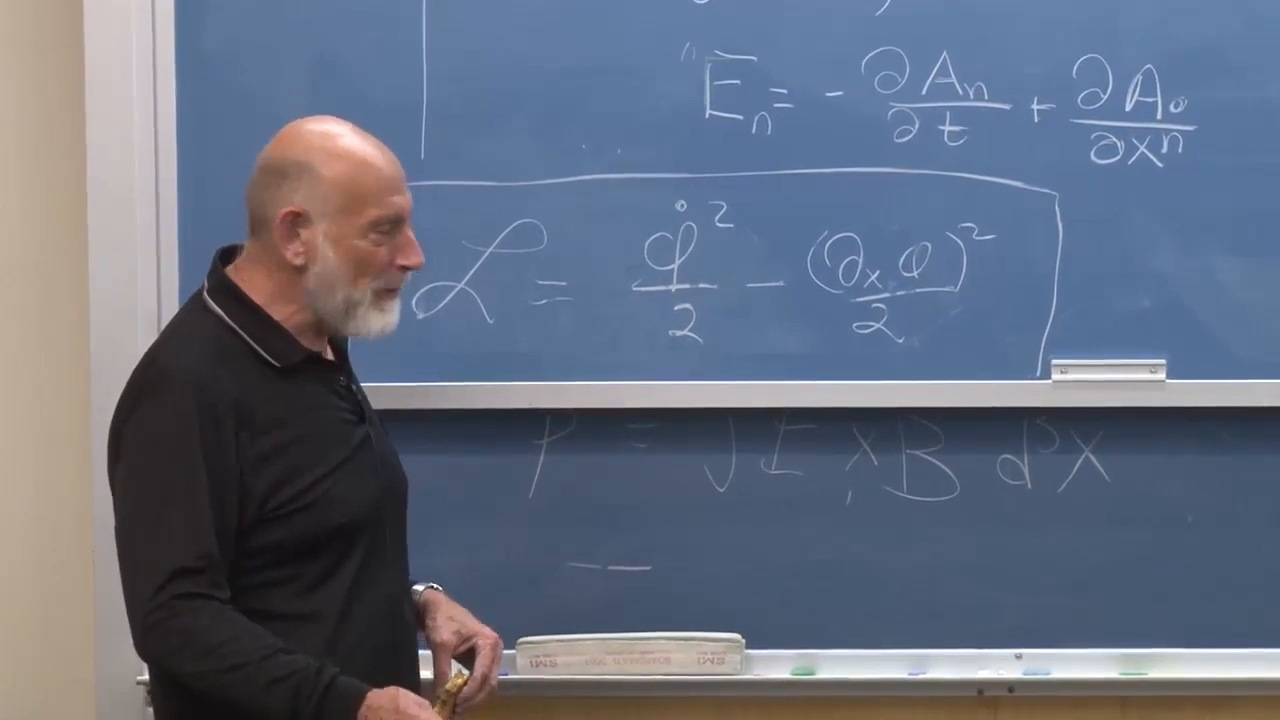
\includegraphics[width=\linewidth]{../../figures/lecture_10_figure_27.png}
\caption{The general electric-field relation restored after the
temporal-gauge calculation, together with the covariant scalar
Lagrangian recalled below it.}
\par\smallskip
\textit{Lecture frame: 01:45:40.}
\end{figure}

\begin{classroomqa}
\audiencequestion{Exactly where do the vector potential and the
electric and magnetic fields connect?}
\lecturerresponse{The electric field combines the time derivative of
the spatial potential with the spatial derivative of \(A_0\); the
magnetic field is the curl of the spatial potential. In temporal gauge
this becomes simply
\(\mathbf E=-\dot{\mathbf A}\) and
\(\mathbf B=\nabla\times\mathbf A\).
\lecturetimestamp{01:44:15}}
\end{classroomqa}

\begin{classroomqa}
\audiencequestion{Is the potential more fundamental than
\(\mathbf E\) and \(\mathbf B\)?}
\lecturerresponse{The action and gauge principle are most naturally
formulated with \(A_\mu\), which makes the potential structurally
fundamental. Yet \(A_\mu\) is not unique: gauge-related potentials
represent the same physics, and the local fields are gauge invariant.
The two statements are compatible. Fundamental variables need not
themselves be directly observable. \lecturetimestamp{01:46:36}}
\end{classroomqa}

\begin{classroomqa}
\audiencequestion{Can the gauge potential itself exert a force?}
\lecturerresponse{A gauge-dependent representative cannot produce a
gauge-dependent measurable force. Charged matter is coupled through the
potential in the action, but the classical Lorentz force can be written
entirely in terms of the gauge-invariant electric and magnetic fields.
\lecturetimestamp{01:47:49}}
\end{classroomqa}

\begin{classroomqa}
\audiencequestion{If crossed electric and magnetic fields are static,
must their momentum be zero?}
\lecturerresponse{Not necessarily for the field by itself:
\(\mathbf E\times\mathbf B\) can be nonzero even when both fields are
time independent. In a closed static apparatus the complete momentum
budget also includes the charges, currents, supports, and any
mechanical or hidden momentum. The brief classroom answer that the
total must balance is the correct conservation statement; setting the
field contribution alone to zero would be too strong.
\lecturetimestamp{01:48:01}}
\end{classroomqa}

\section{One Tensor, Two Meanings of the Poynting Vector}

The energy--momentum tensor organizes all the densities and fluxes:
\begin{align}
T^{00}&=\text{energy density},
&
T^{0i}&=\text{\(i\)-momentum density},
\nonumber\\
T^{i0}&=\text{energy flux in the \(i\)-direction},
&
T^{ij}&=\text{\(j\)-momentum flux in the \(i\)-direction}.
\label{eq:stress-energy-components}
\end{align}
For example, \(T^{31}\) is the amount of \(x\)-momentum crossing a unit
area whose normal points in the \(z\)-direction per unit time. The
spatial block \(T^{ij}\) is the stress tensor.

\begin{figure}[H]
\centering
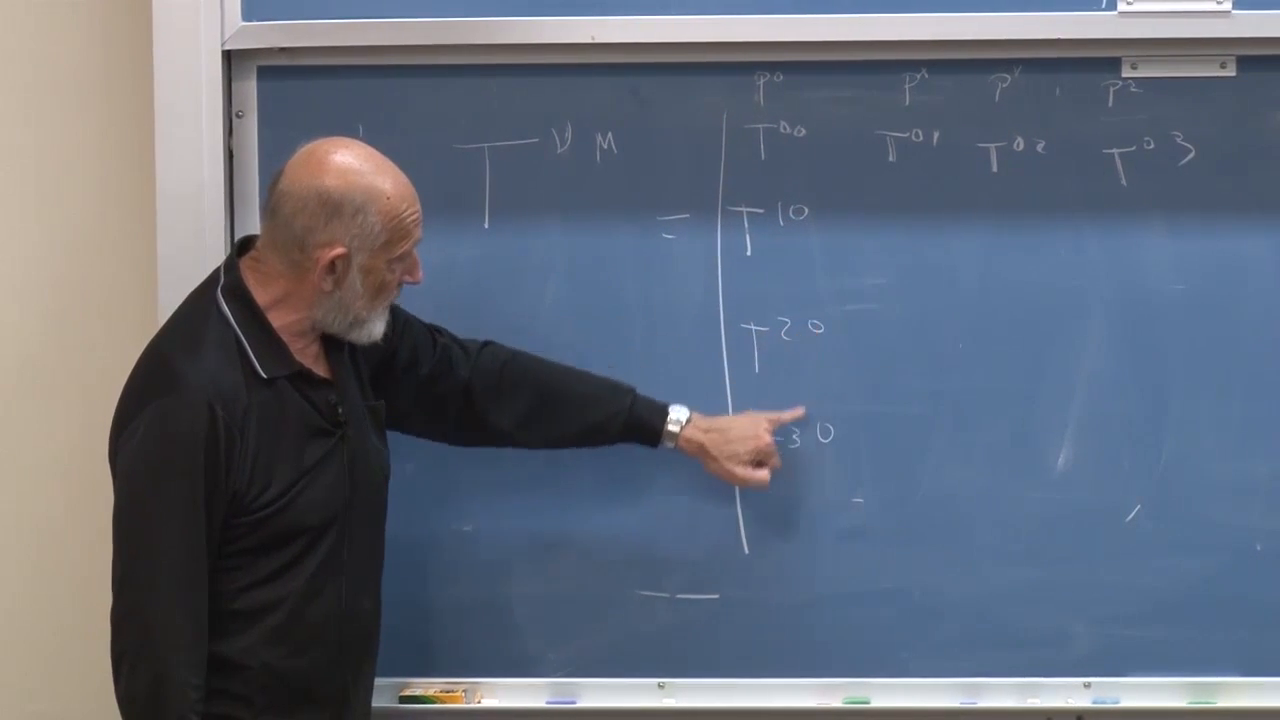
\includegraphics[width=\linewidth]{../../figures/lecture_10_figure_28.png}
\caption{The board begins arranging density and flux components into
the energy--momentum tensor.}
\par\smallskip
\textit{Lecture frame: 01:51:10.}
\end{figure}

For the relativistic systems under discussion, the physical
energy--momentum tensor can be chosen symmetric:
\begin{equation}
T^{\mu\nu}=T^{\nu\mu}.
\label{eq:stress-energy-symmetry}
\end{equation}
Consequently,
\begin{equation}
T^{0i}=T^{i0}.
\label{eq:momentum-density-energy-flux}
\end{equation}
The density of \(i\)-momentum equals the flux of energy in the
\(i\)-direction when \(c=1\). This is the answer to a final audience
memory: the Poynting vector is indeed a power density.

\begin{classroomqa}
\audiencequestion{Is \(\mathbf E\times\mathbf B\) the power density
rather than the momentum density?}
\lecturerresponse{It is both. Symmetry of \(T^{\mu\nu}\) identifies the
momentum density \(T^{0i}\) with the energy flux \(T^{i0}\). Thus
\(\mathbf S=\mathbf E\times\mathbf B\) is energy per unit time per unit
area and, in \(c=1\) units, momentum per unit volume. With ordinary
units restored, \(\mathbf g=\mathbf S/c^2\).
\lecturetimestamp{01:48:20}}
\end{classroomqa}

\begin{figure}[H]
\centering
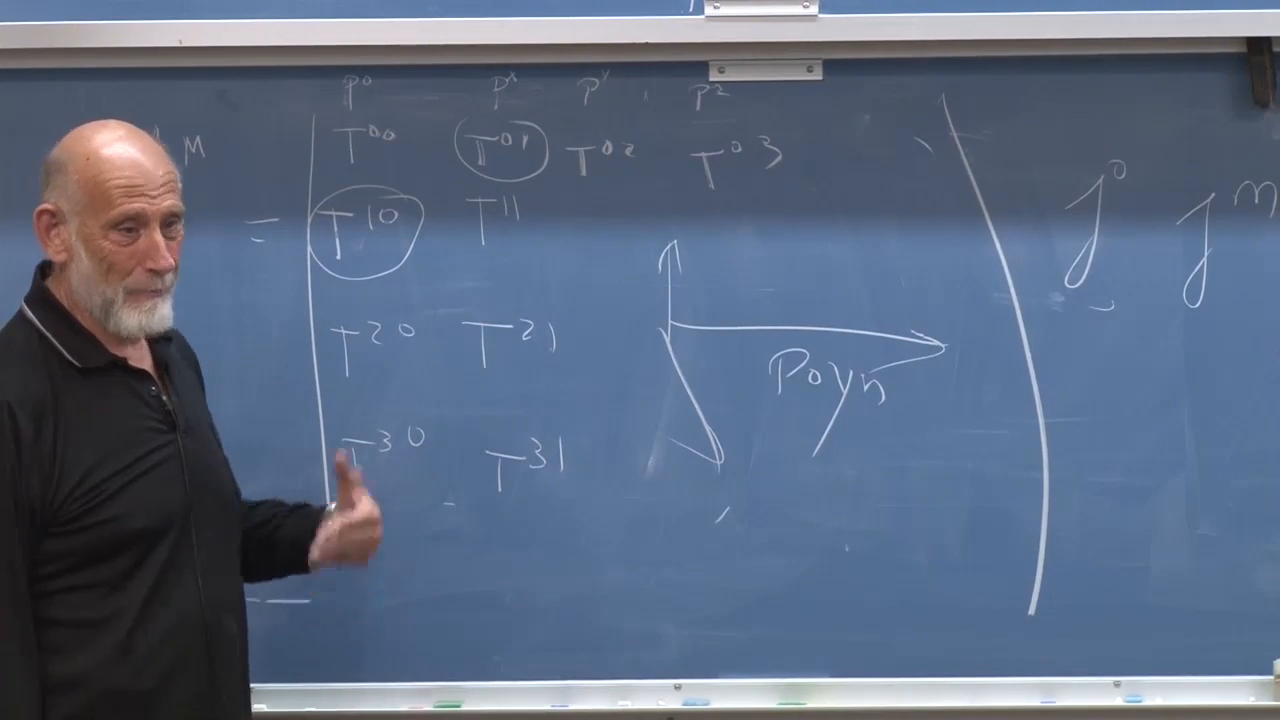
\includegraphics[width=\linewidth]{../../figures/lecture_10_figure_29.png}
\caption{The symmetric tensor relation equating momentum density with
energy flux, labeled on the board by the Poynting vector.}
\par\smallskip
\textit{Lecture frame: 01:53:50.}
\end{figure}

\section{The Bridge to General Relativity}

The course closes by bringing classical mechanics, field theory, and
electromagnetism into one structure:
\begin{enumerate}
\item Time-translation invariance gives the Hamiltonian and energy.
\item Spatial-translation invariance gives Noether momentum.
\item Replacing discrete coordinates by spatially labeled fields turns
sums into integrals and conserved quantities into local densities.
\item Gauge fixing exposes the mechanical coordinates of the Maxwell
field without changing its observables.
\item The Maxwell Hamiltonian gives
\(\frac12(\mathbf E^2+\mathbf B^2)\), while spatial translations give
\(\mathbf E\times\mathbf B\).
\item The symmetric energy--momentum tensor unifies energy density,
momentum density, energy flux, and stress.
\end{enumerate}

This is the quantity needed at the next stage. In general relativity,
the energy--momentum tensor appears as the source in Einstein's field
equation. The final lecture has therefore not merely appended an
electromagnetic calculation; it has prepared the language in which
matter and fields tell spacetime how to curve.
